\documentclass[a4paper, openany]{book}
%\documentclass{tuftebook}
\usepackage{amsthm}
\usepackage[many]{tcolorbox}

\makeatletter

\makeatletter

\def\renewtheorem#1{%
	\expandafter\let\csname#1\endcsname\relax
	\expandafter\let\csname c@#1\endcsname\relax
	\gdef\renewtheorem@envname{#1}
	\renewtheorem@secpar
}
\def\renewtheorem@secpar{\@ifnextchar[{\renewtheorem@numberedlike}{\renewtheorem@nonumberedlike}}
\def\renewtheorem@numberedlike[#1]#2{\newtheorem{\renewtheorem@envname}[#1]{#2}}
\def\renewtheorem@nonumberedlike#1{
	\def\renewtheorem@caption{#1}
	\edef\renewtheorem@nowithin{\noexpand\newtheorem{\renewtheorem@envname}{\renewtheorem@caption}}
	\renewtheorem@thirdpar
}
\def\renewtheorem@thirdpar{\@ifnextchar[{\renewtheorem@within}{\renewtheorem@nowithin}}
\def\renewtheorem@within[#1]{\renewtheorem@nowithin[#1]}

\makeatother

%%%%%%%%%%%%%%%%%%%%
% New environments %
%%%%%%%%%%%%%%%%%%%%

\makeatother
%\mdfsetup{skipabove=1em,skipbelow=0em}

\tcbuselibrary{skins}

% Color definitions

\definecolor{proofcolor}{RGB}{0,0,0}

% Dark orange and Dark Red rgb
\definecolor{theorembordercolor}{RGB}{151, 63, 5}
\definecolor{theorembackgroundcolor}{RGB}{248, 241, 234}

\definecolor{examplebordercolor}{RGB}{0, 110, 184}
\definecolor{examplebackgroundcolor}{RGB}{240, 244, 250}

\definecolor{definitionbordercolor}{RGB}{0, 150, 85}
\definecolor{definitionbackgroundcolor}{RGB}{239, 247, 243}

\definecolor{propertybordercolor}{RGB}{128, 0, 128}
\definecolor{propertybackgroundcolor}{RGB}{255, 240, 255}

\definecolor{formulabordercolor}{RGB}{0, 0, 0}
\definecolor{formulabackgroundcolor}{RGB}{230, 229, 245}

\newtheoremstyle{theorem}
{0pt}{0pt}{\normalfont}{0pt}
{}{\;}{0.25em}
{{\sffamily\bfseries\color{theorembordercolor}\thmname{#1}~\thmnumber{\textup{#2}}.}
	\thmnote{\normalfont\color{black}~(#3)}}

\newtheoremstyle{definition}
{0pt}{0pt}{\normalfont}{0pt}
{}{\;}{0.25em}
{{\sffamily\bfseries\color{definitionbordercolor}\thmname{#1}~\thmnumber{\textup{#2}}.}
	\thmnote{\normalfont\color{black}~(#3)}}

\newtheoremstyle{example}
{0pt}{0pt}{\normalfont}{0pt}
{}{\;}{0.25em}
{{\sffamily\bfseries\color{examplebordercolor}\thmname{#1}.}
	\thmnote{\normalfont\color{black}~(#3)}}

\newtheoremstyle{property}
{0pt}{0pt}{\normalfont}{0pt}
{}{\;}{0.25em}
{{\sffamily\bfseries\color{propertybordercolor}\thmname{#1}~\thmnumber{\textup{#2}}.}
	\thmnote{\normalfont\color{black}~(#3)}}

\newtheoremstyle{formula}
{0pt}{0pt}{\normalfont}{0pt}
{}{\;}{0.25em}
{{\sffamily\bfseries\color{formulabordercolor}\thmname{#1}~\thmnumber{\textup{#2}}.}
	\thmnote{\normalfont\color{black}~(#3)}}

%%%%%%%%%%%%%%%%%%%%%%%%
% Theorem Environments %
%%%%%%%%%%%%%%%%%%%%%%%%

\theoremstyle{theorem}

\newtheorem{theorem}{Theorem}
\newtheorem{postulate}{Postulate}
\newtheorem{conjecture}{Conjecture}
\newtheorem{corollary}{Corollary}
\newtheorem{lemma}{Lemma}
\newtheorem{conclusion}{Conclusion}

\tcolorboxenvironment{theorem}{
	enhanced jigsaw, pad at break*=1mm, breakable,
	left=4mm, right=4mm, top=1mm, bottom=1mm,
	colback=theorembackgroundcolor, boxrule=0pt, frame hidden,
	borderline west={0.5mm}{0mm}{theorembordercolor}, arc=.5mm
}
\tcolorboxenvironment{postulate}{
	enhanced jigsaw, pad at break*=1mm, breakable,
	left=4mm, right=4mm, top=1mm, bottom=1mm,
	colback=theorembackgroundcolor, boxrule=0pt, frame hidden,
	borderline west={0.5mm}{0mm}{theorembordercolor}, arc=.5mm
}
\tcolorboxenvironment{conjecture}{
	enhanced jigsaw, pad at break*=1mm, breakable,
	left=4mm, right=4mm, top=1mm, bottom=1mm,
	colback=theorembackgroundcolor, boxrule=0pt, frame hidden,
	borderline west={0.5mm}{0mm}{theorembordercolor}, arc=.5mm
}
\tcolorboxenvironment{corollary}{
	enhanced jigsaw, pad at break*=1mm, breakable,
	left=4mm, right=4mm, top=1mm, bottom=1mm,
	colback=theorembackgroundcolor, boxrule=0pt, frame hidden,
	borderline west={0.5mm}{0mm}{theorembordercolor}, arc=.5mm
}
\tcolorboxenvironment{lemma}{
	enhanced jigsaw, pad at break*=1mm, breakable,
	left=4mm, right=4mm, top=1mm, bottom=1mm,
	colback=theorembackgroundcolor, boxrule=0pt, frame hidden,
	borderline west={0.5mm}{0mm}{theorembordercolor}, arc=.5mm
}
\tcolorboxenvironment{conclusion}{
	enhanced jigsaw, pad at break*=1mm, breakable,
	left=4mm, right=4mm, top=1mm, bottom=1mm,
	colback=theorembackgroundcolor, boxrule=0pt, frame hidden,
	borderline west={0.5mm}{0mm}{theorembordercolor}, arc=.5mm
}

%%%%%%%%%%%%%%%%%%%%%%%%%%%
% Definition Environments %
%%%%%%%%%%%%%%%%%%%%%%%%%%%

\theoremstyle{definition}
\newtheorem{definition}{Definition}
\newtheorem{review}{Review}

\tcolorboxenvironment{definition}{
	enhanced jigsaw, pad at break*=1mm, breakable,
	left=4mm, right=4mm, top=1mm, bottom=1mm,
	colback=definitionbackgroundcolor, boxrule=0pt, frame hidden,
	borderline west={0.5mm}{0mm}{definitionbordercolor}, arc=.5mm
}
\tcolorboxenvironment{review}{
	enhanced jigsaw, pad at break*=1mm, breakable,
	left=4mm, right=4mm, top=1mm, bottom=1mm,
	colback=definitionbackgroundcolor, boxrule=0pt, frame hidden,
	borderline west={0.5mm}{0mm}{definitionbordercolor}, arc=.5mm
}


%%%%%%%%%%%%%%%%%%%%%%%%
% Example Environments %
%%%%%%%%%%%%%%%%%%%%%%%%

\theoremstyle{example}
\newtheorem*{example}{Example}
\newtheorem*{remark}{Remark}
\newtheorem*{note}{Note}

\tcolorboxenvironment{example}{
	enhanced jigsaw, pad at break*=1mm, breakable,
	left=4mm, right=4mm, top=1mm, bottom=1mm,
	colback=examplebackgroundcolor, boxrule=0pt, frame hidden,
	borderline west={0.5mm}{0mm}{examplebordercolor}, arc=.5mm
}
\tcolorboxenvironment{remark}{
	enhanced jigsaw, pad at break*=1mm, breakable,
	left=4mm, right=4mm, top=1mm, bottom=1mm,
	colback=white, boxrule=0pt, frame hidden,
	borderline west={0.5mm}{0mm}{examplebordercolor}, arc=.5mm
}
\tcolorboxenvironment{note}{
	enhanced jigsaw, pad at break*=1mm, breakable,
	left=4mm, right=4mm, top=1mm, bottom=1mm,
	colback=white, boxrule=0pt, frame hidden,
	borderline west={0.5mm}{0mm}{examplebordercolor}, arc=.5mm
}


%%%%%%%%%%%%%%%%%%%%%%%%%
% Property Environments %
%%%%%%%%%%%%%%%%%%%%%%%%%

\theoremstyle{property}
\newtheorem{property}{Property}
\newtheorem{proposition}{Proposition}

\tcolorboxenvironment{property}{
	enhanced jigsaw, pad at break*=1mm, breakable,
	left=4mm, right=4mm, top=1mm, bottom=1mm,
	colback=propertybackgroundcolor, boxrule=0pt, frame hidden,
	borderline west={0.5mm}{0mm}{propertybordercolor}, arc=.5mm
}
\tcolorboxenvironment{proposition}{
	enhanced jigsaw, pad at break*=1mm, breakable,
	left=4mm, right=4mm, top=1mm, bottom=1mm,
	colback=propertybackgroundcolor, boxrule=0pt, frame hidden,
	borderline west={0.5mm}{0mm}{propertybordercolor}, arc=.5mm
}

%%%%%%%%%%%%
% Formula %
%%%%%%%%%%%%

\theoremstyle{formula}
\newtheorem{formula}{Formula}

\tcolorboxenvironment{formula}{
	enhanced jigsaw, pad at break*=1mm, breakable,
	left=4mm, right=4mm, top=1mm, bottom=1mm,
	colback=formulabackgroundcolor, boxrule=0pt, frame hidden,
	borderline west={0.5mm}{0mm}{formulabordercolor}, arc=.5mm
}

%%%%%%%%%
% Proof %
%%%%%%%%%

% These patches must be placed after \tcolorboxenvironment !
\AddToHook{env/theorem/after}{\colorlet{proofcolor}{theorembordercolor}}
\AddToHook{env/postulate/after}{\colorlet{proofcolor}{theorembordercolor}}
\AddToHook{env/conjecture/after}{\colorlet{proofcolor}{theorembordercolor}}
\AddToHook{env/corollary/after}{\colorlet{proofcolor}{theorembordercolor}}
\AddToHook{env/lemma/after}{\colorlet{proofcolor}{theorembordercolor}}
\AddToHook{env/conclusion/after}{\colorlet{proofcolor}{theorembordercolor}}

\AddToHook{env/definition/after}{\colorlet{proofcolor}{definitionbordercolor}}
\AddToHook{env/review/after}{\colorlet{proofcolor}{definitionbordercolor}}

\AddToHook{env/example/after}{\colorlet{proofcolor}{examplebordercolor}}
\AddToHook{env/remark/after}{\colorlet{proofcolor}{examplebordercolor}}
\AddToHook{env/note/after}{\colorlet{proofcolor}{examplebordercolor}}

\AddToHook{env/property/after}{\colorlet{proofcolor}{propertybordercolor}}
\AddToHook{env/proposition/after}{\colorlet{proofcolor}{propertybordercolor}}

\AddToHook{env/formula/after}{\colorlet{proofcolor}{formulabordercolor}}

\renewcommand{\qedsymbol}{Q.E.D.}
\let\qedsymbolMyOriginal\qedsymbol
\renewcommand{\qedsymbol}{
	\color{proofcolor}\qedsymbolMyOriginal
}

\newtheoremstyle{proof}
{0pt}{0pt}{\normalfont}{0pt}
{}{\;}{0.25em}
{{\sffamily\bfseries\color{proofcolor}\thmname{#1}.}
	\thmnote{\normalfont\color{black}~(\textit{#3})}}

\theoremstyle{proof}
\renewtheorem{proof}{Proof}

\tcolorboxenvironment{proof}{
	enhanced jigsaw, pad at break*=1mm, breakable,
	left=4mm, right=4mm, top=1mm, bottom=1mm,
	colback=white, boxrule=0pt, frame hidden,
	borderline west={0.5mm}{0mm}{proofcolor}, arc=.5mm
}

\newenvironment{info}{\begin{tcolorbox}[
		arc=0mm,
		colback=white,
		colframe=gray,
		title=Info,
		fonttitle=\sffamily,
		breakable
		]}{\end{tcolorbox}}
\newenvironment{terminology}{\begin{tcolorbox}[
		arc=0mm,
		colback=white,
		colframe=green!60!black,
		title=Terminology,
		fonttitle=\sffamily,
		breakable
		]}{\end{tcolorbox}}
\newenvironment{warning}{\begin{tcolorbox}[
		arc=0mm,
		colback=white,
		colframe=red,
		title=Warning,
		fonttitle=\sffamily,
		breakable
		]}{\end{tcolorbox}}
\newenvironment{caution}{\begin{tcolorbox}[
		arc=0mm,
		colback=white,
		colframe=yellow,
		title=Caution,
		fonttitle=\sffamily,
		breakable
		]}{\end{tcolorbox}}

\begin{document}
\begin{titlepage}
    \begin{center}
        \line(1,0){300} \\
        [0.25in]
        \huge{\bfseries Math 210A Notes} \\
        [2mm]
        \line(1,0){200} \\
        [1.5cm]
        \textsc{\LARGE Fall, 2025}
    \end{center}
\end{titlepage}

\tableofcontents
\setcounter{section}{0}

\chapter{Preliminaries}
\section{Groups, Permutations and Cycle Decompositions}
\begin{definition}(Group) \leavevmode \\
    A group is an ordered pair $(G, *)$ where $G$ is a set and $*$ is a mapping from $G\times G$ to $G$ (called a binary operation) satisfying the following:
    \begin{enumerate}
        \item $\forall a, b, c \in G ~~a*(b*c)=(A*b)*c$ (associativity)
        \item $\exists e \in G \st e*a=a=a*e ~~\forall a \in G$ (identity element)
        \item $\forall a \in G, \exists a^{-1} \in G \st a*a^{-1}=e=a^{-1}*a$ (inverse element)
    \end{enumerate}
\end{definition}

From now on we write $a*b = ab$.

\begin{definition}[Permutations] \leavevmode \\
    Let $\Omega$ be a nonempty set. The mapping $\sigma: \Omega \to \Omega$ is a permutation of $\Omega$ if $\sigma$ is a bijection.
\end{definition} %
\begin{wrapfigure}{l}{0.35\textwidth} % l = left, r = right
  \centering
  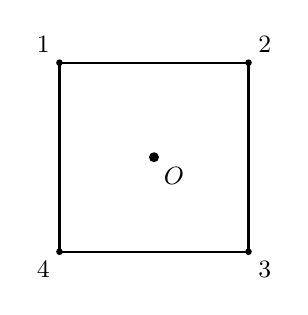
\begin{tikzpicture}[scale=1.2, every node/.style={font=\small}]
    % square centered at origin
    \coordinate (A) at (-1,-1); % 1
    \coordinate (B) at ( 1,-1); % 2
    \coordinate (C) at ( 1, 1); % 3
    \coordinate (D) at (-1, 1); % 4
    \draw[thick] (A) -- (B) -- (C) -- (D) -- cycle;

    % vertex dots + labels
    \fill (A) circle (1pt); \node[below left]  at (A) {4};
    \fill (B) circle (1pt); \node[below right] at (B) {3};
    \fill (C) circle (1pt); \node[above right] at (C) {2};
    \fill (D) circle (1pt); \node[above left]  at (D) {1};

    % origin
    \fill (0,0) circle (1.5pt);
    \node[below right] at (0,0) {$O$};
  \end{tikzpicture}
\end{wrapfigure}

Here is a square centered at the origin. Take a copy of the square, move it around in 3-space, and lay it back down to cover the original square. This is called a rigid motion of the square, or a symmetry of the square. This creates a permutation of the vertices. How many symmetries are possible?

%%%%%%%%%%%%%%%%figures go here %%%%%%%%%%%%%%%%

For the arbitrary symmetry of the square, we have 4 choices where to find 1. Once we know where vertex 1 is (say, vertex i), then vertex 2 can be one of 2 places. This gives $4\times2$ symmetries. Consider the regular $n$-gon centered at the origin. How many symmetries do we have? $2n$.

\begin{fact} [Properties of Permutations] \leavevmode \\
\begin{enumerate}
    \item Functional composition is associative. For mappings $\sigma, \tau, \mu$
    $$\sigma \circ (\tau \circ \mu) = (\sigma \circ \tau) \circ \mu$$
    \item The identity mapping on any set ($I(x) = x$) is a bijection of that set.
    \item If $\sigma$ is a bijection from a set $\Omega$ to $\Omega$, then there is a bijection of $\Omega$ called $\sigma^{-1}$ such that $\sigma \circ \sigma^{-1} = I = \sigma^{-1} \circ \sigma$.
\end{enumerate}
\end{fact}

\begin{definition}[Order] \leavevmode \\
    For $a\in G$, where $G$ is a group, the order of $a$, denoted $|a|$, is the smallest positive integer $k$ such that $a^k = e$ if such a $k$ exists. If no such $k$ exists, then we say $a$ has infinite order and $|a| = \infty$.
\end{definition}

\begin{notation}[Cycle Decomposition] \leavevmode \\
    A permutation $\sigma$ of a set $\Omega$ can be written as a product of disjoint cycles. For example, if $\sigma$ is a permutation of $\{1,2,3,4,5\}$ such that $\sigma(1)=3$, $\sigma(3)=1$, $\sigma(2)=5$, $\sigma(5)=2$, and $\sigma(4)=4$, then we can write $\sigma = (1~3)(2~5)(4)$. The order of a cycle is the number of elements in the cycle. The order of a permutation is the least common multiple of the orders of the disjoint cycles.
\end{notation}

\begin{example} \leavevmode \\
  If $\sigma = (1~2)(3~2),$ then $\sigma(3) = 1$. \\
  If $\mu = (3~2)(1~2),$ then $\mu(3) = 2$. \\
  $S_n$ is not abelian for $n \geq 3$.
\end{example}

\newpage

\section{Orders of Permutations}
$S_X$ refers to the set of all permutations on the set $X$. That is, the elements of $S_X$ are bijections from $X$ to itself. $S_n$ refers to when $X=\set{1,2,\ldots,n}.$

Let $n=5$. How many elements are in $S_5$? $5!=120$. Why? Given a $\sigma \in S_5$, we have $5$ choices for $\sigma(1)$, 4 for $\sigma(2),...$ so there are $5\cdot 4 \cdot 3 \cdot 2 \cdot 1=5! = 120$ choices for $\sigma$. In general, there $n!$ elements in $S_n$.

$S_5:$ how many cycles of length $5$ are in $S_5$?

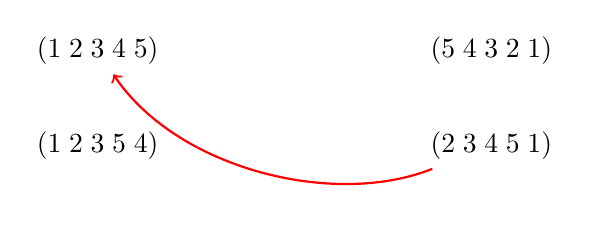
\begin{tikzpicture}[baseline=(current bounding box.center)]
\node (a) at (0,0) {$(1\;2\;3\;4\;5)$};
\node (b) at (5,0) {$(5\;4\;3\;2\;1)$};
\node (c) at (0,-1.2) {$(1\;2\;3\;5\;4)$};
\node (d) at (5,-1.2) {$\cancel{(2\;3\;4\;5\;1)}$};
\draw[->, red, thick] (d) .. controls (3,-2) and (1,-1.5) .. (a);
\end{tikzpicture} 

$\vdots$

There are $5!$ ways of filling in a blank 5-cycle. However, each 5-cycle is represented 5 ways, so we divide by 5. Thus there are $\frac{5!}{5} = 4! = 24$ distinct 5-cycles in $S_5$.How many
\begin{align*}
    \text{4 cycles? } & \frac{5\cdot4\cdot3\cdot2}{4} = 30 \\
    \text{3 cycles? } & \frac{5\cdot4\cdot3}{3} = 20 \\
    \text{2 cycles? } & \frac{5\cdot4}{2} = 10 \\
    \text{1 cycles? } & \frac{5}{1} = 5
\end{align*}

How many distinct $r$-cycles $r \leq n$ are there in $S_n$? $\frac{n!}{r(n-r)!}$
$$\frac{n\cdot(n-1)\cdot(n-2)\cdots(n-r+1)}{r!}$$

How many distinct elements of the form $(\_ \_)(\_ \_ \_)$ disjoint in $S_5$?
$$\frac{5\cdot4}{2} \cdot \frac{3\cdot2\cdot1}{3} = 20$$

How many of the form $(\_ \_)(\_ \_)$?
$$\frac{\frac{5\cdot4}{2} \cdot \frac{3\cdot2}{2}}{2} = \frac{30}{2}=15$$

How many distinct elements of the form $(\_ \_)(\_ \_ \_)$ in $S_n$?
$$\frac{n\cdot(n-1)}{2} \cdot \frac{(n-2)(n-3)(n-4)}{3}$$

How many distinct elements of the form $(\_ \_)(\_ \_)$ in $S_n$?
$$\frac{\frac{n\cdot(n-1)}{2} \cdot \frac{(n-2)(n-3)}{2}}{2}$$

\begin{definition}[Field] \leavevmode \\
    $(F, +, \cdot)$ is a field if
    \begin{enumerate}
        \item $(F, +)$ is an abelian group with identity $0$
        \item $(F\setminus\set{0}, \cdot)$ is an abelian group with identity $1$
        \item Left and right distributive laws hold
    \end{enumerate}
\end{definition}

The following are groups:
\begin{align*}
    GL_n(F) &= \set{\text{all $n\times n$ matrices with entries in $F$ and with non-zero determinants}} \\
    SL_n(F) &= \set{\text{all $n\times n$ matrices with entries in $F$ and with determinant $1$}}
\end{align*}
\newpage

\section{Homomorphism and Isomorphism}
In general, we can tell how similar groups are by the mappings we make between them where the mappings preserve the group structure of the domain.

\begin{definition}[Homomorphism] \leavevmode \\
    Let $(G, \star)$ and $(H, \diamond)$ be groups. A map $\Phi: G \to H$ is a homomorphism if for all $g_1, g_2 \in G$,
    $$\Phi(g_1 \star g_2) = \Phi(g_1) \diamond \Phi(g_2)$$
    We usually write
    $$\Phi(xy) = \Phi(x) \Phi(y)$$
    and we know that $xy$ happens in $G$ and $\Phi(x)\Phi(y)$ happens in $H$.
\end{definition}

\begin{example}
    $\pi: \R^2 \to \R$ by $\pi(x,y) = x$ $\forall (x,y) \in \R^2$ is a homomorphism. Letting $(x_1, y_1), (x_2, y_2) \in \R^2$, we have
    \begin{align*}
        \pi((x_1, y_1) + (x_2, y_2)) &= \pi(x_1 + x_2, y_1 + y_2) \\
        &= x_1 + x_2 \\
        &= \pi(x_1, y_1) + \pi(x_2, y_2)
    \end{align*}
    Showing that $\pi$ is indeed a homomorphism.

    What elements are in the set $\set{p \in \R^2 : \pi(p) = 0} = K$?
    $$K = \set{(x,y) : x=0}$$
    This is the kernel of $\pi$.
\end{example}

\begin{definition}[Kernel] \leavevmode \\
    Let $G$ and $H$ be groups and let $\Phi: G \to H$ be a group homomorphism. The kernel of $\Phi$ is
    $$\ker(\Phi) = \set{g \in G : \Phi(g) = e_H} = \Phi^{-1}(e_H)$$
    where $e_H$ is the identity element in $H$.
\end{definition}

\begin{definition}[Isomorphism] \leavevmode \\
    Let $G$ and $H$ be groups. A map $\Psi: G \to H$ is an isomorphism if
    \begin{enumerate}
        \item $\Psi$ is a homomorphism
        \item $\Psi$ is bijective
    \end{enumerate}
    If there exists an isomorphism $\Psi: G \to H$, we say that $G$ and $H$ are isomorphic, denoted $G \cong H$.
    
    $\cong$ is an equivalence relation on any collection of groups.
\end{definition}

\begin{example}
    Let $k \in \Q^\ast = \Q \setminus \set{0}$. Define $\phi_k: \Q^\ast \to \Q^\ast$ by $\phi_k(q) = kq$. We claim that $\phi$ is an isomorphism.
    Show that $\Phi_k$ is a homomorphism and a bijection:
    \begin{enumerate}
        \item Homomorphism:
        \begin{align*}
            \phi_k(q_1 + q_2) &= k(q_1 +q_2) \\
            &= k (q_1+ q_2) \\
            &= kq_1 + kq_2 \\
            &= \phi_k(q_1) + \phi_k(q_2)
        \end{align*}
        \item Bijections:
        \begin{itemize}
            \item Injective: Suppose $\phi_k(q_1) = \phi_k(q_2)$. Then \begin{align*}
                \phi_k(q_1) &= \phi_k(q_2) \\ \iff
                kq_1 &= kq_2 \\ \iff
                q_1 &= q_2 &&(k \neq 0)
            \end{align*}
            \item Surjective: We want to show $\phi_k(\Q) = \Q$. Let $q \in \Q.$ Since $k \neq 0$, $\frac{q}{k} \in \Q$. Then
            $$\phi_k\left(\frac{q}{k}\right) = k \cdot \frac{q}{k} = q$$
            Thus $\phi_k$ is surjective.
        \end{itemize}
    \end{enumerate}
    ker$\phi_k=\set{0}$ since $\phi_k(q) = 0 \iff kq = 0 \iff q=0$.
\end{example}

\begin{fact}
    Suppose $G \cong H,$ that is there exists $\phi: G \to H$ which is a homomorphic bijection. Then
    \begin{enumerate}
        \item $|G|=|H|$
        \item $G$ is abelian if and only if $|H|$ is abelian
        \item $\forall x \in G ~~|x| = |\phi(x)|$ (Corresponding elements have the same order)
    \end{enumerate}
\end{fact}
\newpage

\section{Group Actions}
There are many examples of groups acting on sets. For instance, consider an element in $S_5$, call it $\sigma.$ $\sigma$ is a permutation of $\set{1,2,3,4,5}$ and it is also an element of a group
\begin{align*}
    \sigma &= (1~2~3~4~5) \\
    &\sigma(5) = 4
\end{align*}
We say that $\sigma$ is acting on the set $\set{1,2,3,4,5}$.

Consider the set of all $2\times 2$ matrices with elements in $\R$. Let $A = \begin{bmatrix}
1 & 2 \\
3 & 4
\end{bmatrix}$ and let $k \in \R.$ Then $kA = \begin{bmatrix}
k & 2k \\
3k & 4k
\end{bmatrix}.$ We say that $\R$ is acting on the set of all $2\times 2$ matrices with elements in $\R$.

\begin{definition}[Group Action] \leavevmode \\
    Let $G$ be a group and $A$ be a set. A group action of $G$ on $A$ is a map from $G\times A$ to $A$ (written $g.a ~~\forall g \in G, a \in A$) such that
    \begin{enumerate}
        \item $g_1.(g_2.a) = (g_1g_2).a ~~\forall g_1, g_2 \in G$ (Compatability)
        \item $1.a = a$ (or $e.a = a$) $ ~~\forall a \in A$ (Identity)
    \end{enumerate}
\end{definition}

\begin{example}
    Let $G = S_n$. Let's verify that $S_n$ acts on the set $\set{1,2,...,n}.$ Define the group action
    \begin{align*} \tag{$*$}
        \sigma.a = \sigma(a) ~~\forall \sigma \in S_n, a \in \set{1,2,...,n}
    \end{align*}
    Then let $\sigma_1, \sigma_2 \in S_n$ and $a \in \set{1,2,...,n}.$ We have
    \begin{align*}
        \sigma_1.(\sigma_2.a) &= \sigma_1.(\sigma_2(a)) \\
        &= \sigma_1(\sigma_2(a)) \\
        &= (\sigma_1\circ\sigma_2)(a) \\
        &= (\sigma_1\circ\sigma_2).a \tag{I}
    \end{align*}
    To verify the identity property, recall that the identity map, denoted $I$, is the identity of $S_n$ and $$I(a) = a ~~\forall a \in \set{1,2,...,n}$$
    That is,
    \begin{align*}
        I.a = I(a) = a ~~\forall a \in \set{1,2,...,n} \tag{II}
    \end{align*}
    By $(I)$ and $(II)$, $S_n$ acts on the set $\set{1,2,...,n}$ by the group action defined in $(*)$.
\end{example}

\begin{example}
    A vector space over a field $F$ is a set $V$ with two binary operations vector addition and scalar multiplication, and other poperties including 
    \begin{itemize}
        \item $a(bv) = (ab)v ~~\forall a, b \in F, v \in V$ (Compatability)
        \item $1v = v ~~\forall v \in V$ where $1$ is the multiplicative identity in $F$ (Identity)
    \end{itemize}
    Since $F$ is not a group with respect to multiplication, we must say that $F^\ast = F \setminus \set{0}$ acts on $V$.
\end{example}
\newpage

\section{Permutations and Group Actions}
Let $G$ be a group acting on a set $S$. That is, define a mapping $G \times S \to S$ denoted by $g.a ~~\forall g \in G$ and $a \in S$. Fix $g \in G.$ Then this defines a map $\sigma_g \st \sigma_g : S \to S$ by $\sigma_g (a) = g.a$

\begin{example}
    Take $G = \R \setminus \set{0}$ with respect to multiplication. Let $S = M_2(\R)$.
    \begin{align*}
        \sigma_{\sqrt{2}}(A) &= \sqrt{2}.A \\
        &= \sqrt{2} \begin{bmatrix}
            a & b \\
            c & d
        \end{bmatrix} \\
        &= \begin{bmatrix}
            \sqrt{2}a & \sqrt{2}b \\
            \sqrt{2}c & \sqrt{2}d
        \end{bmatrix}
    \end{align*}
    For $\begin{bmatrix}
        1 & \pi \\
        e & \ln(2)
    \end{bmatrix}$, we have
    \begin{align*}
        \sigma_{\sqrt{2}} \begin{bmatrix}
            1 & \pi \\
            e & \ln(2)
        \end{bmatrix} &= \begin{bmatrix}
            \sqrt{2} & \sqrt{2}\pi \\
            \sqrt{2}e & \sqrt{2}\ln(2)
        \end{bmatrix}
    \end{align*}
    What is the range of $\sigma_{\sqrt{2}}$? $M_2(\R)$.
\end{example}

\begin{assertion}
    \begin{enumerate}
        \item $\sigma_g$ as defined is a permutation of the set $S$.
        \item For the sake of notation, we change the name of our set to $A$. The map from $G$ to $S_A$ defined by $g \mapsto \sigma_g$ is a homomorphism.
    \end{enumerate}
\end{assertion}

\begin{proof}
    \begin{enumerate}
        \item Let $g\in G$ be given and $\sigma_g$ be defined as above. Clearly, $\sigma_g$ is a mapping from $S \to S$. We will show that $\sigma_g$ is a bijection by showing it has a two-sided inverse. Let $a \in S$ and note $g^{-1}\in G$ since $G$ is a group. Then
        \begin{align*}
            \left(\sigma_{g^{-1}} \circ \sigma_g \right)(a) &= \sigma_{g^{-1}}(\sigma_g(a)) \\
            &= \sigma_{g^{-1}}(g.a) \\
            &= g^{-1}.(g.a) \\
            &= (g^{-1}g).a \\
            &= e.a \\
            &= a.
        \end{align*}
        We see that $\sigma_{g^{-1}} \circ \sigma_g$ is the identity mapping from $S \to S$. To show that $\sigma_g \circ \sigma_{g^{-1}}$ is also the identity map from $S \to S$ is analogous. Thus we have a two-sided inverse as desired. Hence, $\sigma_g$ is a permutation of $S$ as desired. That is, $\sigma_g$ is an element of the symmetric group of $S$.

        \item Let $\Psi: G \to S_A$ be defined by $\Psi(g) = \sigma_g ~~\forall g \in G$. Let $a \in A$ and $g_1, g_2 \in G$. We want to show that $\Psi(g_1g_2) = \Psi(g_1) \circ \Psi(g_2)$. Since these are mappings in $S_A$, we will show that their values agree $\forall a \in A$. We have
        \begin{align*}
            \left(\Psi(g_1) \circ \Psi(g_2)\right)(a) &= \sigma_{g_1g_2}(a) \\
            &= (g_1g_2).a \\
            &= g_1.(g_2.a) \\
            &= g_1.(\sigma_{g_2}(a)) \\
            &= \sigma_{g_1}(\sigma_{g_2}(a)) \\
            &= \sigma_{g_1} \circ \sigma_{g_2}(a) \\
            &= \left(\Psi(g_1) \circ \Psi(g_2)\right)(a).
        \end{align*}
        Hence, $\Psi$ is a homomorphism as desired.
    \end{enumerate}
    \qed
\end{proof}

If we have a homomorphism, then we have a kernel.

\begin{definition}[Kernel of a Group Action] \leavevmode \\
    For a group $G$ acting on a set $A$, the kernel of the group action is
    $$\set{g \in G : g.a = a ~~\forall a \in A}$$
\end{definition}
\newpage

\chapter{Subgroups}
\section{Subgroups}
\begin{definition} [Subgroup] \leavevmode \\    
    Let $G$ be a group. The subset $H$ of $G$ is called a subgroup of $G$ if 
    \begin{enumerate}
        \item $H$ is nonempty.
        \item $\forall x,y \in H$, $x^{-1} \in H$ and $xy \in H$.
    \end{enumerate}
\end{definition}

\begin{notation}
    IF $H$ is a subgroup of $G$, we write $H \leq G$.
\end{notation}

\begin{example} \leavevmode \\
    \begin{enumerate}
        \item $\Z \leq \Q$ with respect to $(+)$.
        \item All groups have two subgroups: $H=G$ and $H=\set{1}$.
        \item $2\Z \leq \Z$ with respect to $(+)$.
        \item Let $G=D_{2n}$ and let $r$ be a $360^{\circ}/n$ clockwise rotation of the n-gon about the origin. Then $\set{1, r, r^2, r^3,...,r^{n-1}}$ forms a subgroup of $D_{2n}$.
        \item Nonexample: $H=\set{1, -1} \subseteq \Z$ forms a group with respect to multiplicaiton, but $H$ is not a subgroup of $\Z$ since $\Z$ is a group with respect to addition, NOT multiplicaiton.
        \item $\Z/5\Z$ is not a subgroup of $\Z/6\Z$ since $\Z/5\Z \not \subseteq \Z/6\Z$.
        \begin{align*}
            \Z/6\Z &= \set{\bar{0}, \bar{1}, \bar{2}, \bar{3}, \bar{4}, \bar{5}} \text{ is an additive group} \\
            \left(\Z/6\Z\right)^* &= \set{\bar{1}, \bar{5}} \text{ is a multiplicative group with all elements coprime to 6} \\
            \left(\Z/9\Z\right)^{**} &= \set{\bar{1}, \bar{2}, \bar{4}, \bar{5}, \bar{7}, \bar{8}} \text{ is a multiplicative group with all elements coprime to 9}
        \end{align*}
    \end{enumerate}
\end{example}

\begin{proposition}[Subgroup Criterion] \leavevmode \\
    A subset $H$ of a group $G$ is a subgroup of $G$ if and only if
    \begin{enumerate}
        \item $H\not = \emptyset$.
        \item $\forall x,y \in H$, $xy^{-1} \in H$ (in additive notation: $\forall x,y \in H$, $x-y \in H$).
    \end{enumerate}
\end{proposition}
\newpage

\section{Centralizers and Normalizers, Stabilizers and Kernels}
\begin{definition} [Centralizers] \leavevmode \\
    Let $A$ be a nonempty subset of a group $G$. Define the centralizer of $A$ in $G$ to be the set
    \begin{align*}
        C_G(A) &= \{ g \in G : gag^{-1} = g ~~\forall a \in A \} \\
        &= \set{g \in G : ga = ag ~~\forall a \in A}
    \end{align*}
\end{definition}

The centralizer of $A$ in $G$ is the set of all elements in $G$ which commute with every element in $A$.

\begin{theorem}
    $C_G(A) \leq G$.
\end{theorem}

\begin{proof}
    Let $a \in A.$ Then 
    \begin{align*}
        1a1^{-1} &= (1a)1^{-1} \\
        &= a1^{-1} \\
        &= a1 \\
        &= a
    \end{align*}
    Thus, $1 \in C_G(A)$.

    Let $x,y \in C_G(A)$. Then $xax^{-1} = a$ and $yay^{-1}=a.$ Note that
    \begin{equation*}
        yay^{-1} = a \iff a = y^{-1}
        \tag{$*$}
    \end{equation*}
    Now
    \begin{align*}
        (xy^{-1})a(xy^{-1})^{-1} &= xy^{-1}a(y^{-1})^{-1}x^{-1} \\
        &= x(y^{-1}ay)x^{-1} \\
        &\overset{(*)}{=} xax^{-1} \\
        &= a
    \end{align*}
    Hence, $xy^{-1} \in C_G(A)$. Furthermore, $C_G(A) \leq G.$
    \qed
\end{proof}

\begin{notation}
    If $A = \set{a}$, we write $C_G(a)$ instead of $C_G(\set{a})$.
\end{notation}

Why was this unnecessary? From the homework, we know that $G$ acts on the subset $A$ by conjugation. That is, we have a mapping $(.): G\times A \to A$ defined by $g.a = gag^{-1} ~~\forall g \in G, a \in A$ which satisfies both axioms of a group action.

Recall that the kernel of a group action is the kernel of the permutation representation of the group action (PRGA). The PRGA is the Homomorphism induced by the group action
\begin{align*}
    \Psi : G \to S_A \\
    g \mapsto \sigma_g
\end{align*}

\begin{example}
    Find the kernel of $G$ acting on $A \subset G$ by conjugation.
    \begin{align*}
        \set{g \in G : g.a = a ~~ \forall a \in A} &= \set{g \in G : gag^{-1} = a ~~\forall a \in A} \\
        &= C_G(A)
    \end{align*}
\end{example}

Suppose that $A = G$. What is $C_G(G)$?
$$\set{g \in G : gag^{-1}=a ~~\forall a \in G}$$
This set is called the center of $G$ denoted $Z(G)$. Since $Z(G)$ is a special case of $C_G(A)$, we know $Z(G) \leq G$.

\begin{definition}[Normalizer] \leavevmode \\
    Define $gAg^{-1} = \set{gag^{-1} : a \in A}$. We will define the normalizer of $A$ in $G$ to be the set 
    $$N_G(A) = \set{g \in G : gAg^{-1} = A}$$
\end{definition}

We will prove $N_G(A) \leq G$, but not yet.
Notice if $gag^{-1} = a ~~ \forall a \in A$ then $gAg^{-1} = \set{gag^{-1} : a \in A} = \set{a : a \in A} = A$. Hence
$$C_G(A) \subseteq N_G(A)$$

\begin{fact} \leavevmode \\
    \begin{enumerate}
        \item If $G$ is abelian, then $Z(G) = G$ since every element commutes with every other element. That is,
        \begin{align*}
        \forall a,b \in G ~~ab = ba &\iff a = bab^{-1} ~~ \forall a,b \in G \\ &\implies b \in Z(G) ~~\forall b \in G
        \end{align*}
        Similarly, $C_G(A) = N_G(A) = G.$
        \item Consider $A=\set{1, (1 ~2)} \subseteq S_3$. Find $C_{S_3}(A)$. Notice that $1$ commutes with everything in $S_3$, specifically $1$ and $(1~2)$. Also,
        $$(1~2)(1~2)(1~2)^{-1} = (1~2)$$
        so $(1~2)\in C_{S_3}(A)$. Hence, $A \leq C_{S_3}(A)$.
        \begin{theorem}[Lagrange's Theorem] \leavevmode \\
            Let $G$ be a finite group $\left(|G| \in \N\right)$ and let $H \leq G$. Then
            $$|H| \text{ divides } |G|$$
        \end{theorem}
        Since $|A| = 2$ and $A \leq C_{S_3}(A)$, we know $2 \big| |C_{S_3}(A)|$ since $C_{S_3}(A) \leq S_3$.
        $$
        \begin{rcases*}
            |C_{S_3}(A)| \big| |S_3| = 3! = 6 \\
            |A| \big| |C_{S_3}(A)|
        \end{rcases*} \implies |C_{S_3}(A)| \in \set{2, 6}$$.
        Thus, $C_{S_3}= A$ or $C_{S_3}(A) = S_3$. Well,
        \begin{align*}
            (1~2)(1~2~3) = (2~3) \\
            (1~2~3)(1~2) = (1~3)
        \end{align*}
        so $(1~2~3) \not \in C_{S_3}(A)$. It follows that $|C_{S_3}(A)| = 2 \implies C_{S_3}(A) = A.$
    \end{enumerate}
\end{fact}
\newpage

\section{Cyclic Groups}
\begin{definition}[Cyclic Group] \leavevmode\\
    A group $H$ is cyclic if $H$ is generated by a single element. That is,
    $$\exists x \in H \st H = \set{x^n : n \in \Z}$$
    $$\left(\exists x \in H \st H = \set{nx : n \in \Z} \text{ using additive notation}\right)$$
    We write $<x> = H$ ($x$ generates $H$).
\end{definition}

\begin{example}
    \begin{enumerate}
        \item $\Z=<1>=<-1>$
        \item The rotations in $D_{2n}$ are generated by $r$ ($360/n$ clockwise rotation)
        \item $U_4 = {1, -1, i, -i} = <i>$
    \end{enumerate}
\end{example}

\begin{note}
    If $H=<x> = \set{x^n : n \in \Z}$, we define 
    \begin{align*}
        x^0 &= 1 \\
        x^{-n} &= (x^n)^{-1} = (x^{-1})^n \text{ for } n > 0
    \end{align*}
\end{note}

\begin{proposition}
    If $H=<x>$, then $|H| = |x|$. If one side of this equality is infinity, then so is the other. More specifically,
    \begin{enumerate}
        \item If $|x| = n < \infty$, then $x^n = 1$ and $1, x, x^2, ..., x^{n-1}$ are all the distinct elements of $H$.
        \item If $|x| = \infty$, then $x^n \not = 1$ when $n \not = 0$ and $x^a \not = x^b$ for all $a \not = b \in \N$.
    \end{enumerate}
\end{proposition}

\begin{proof}
    Let $|x| = n$.
    \begin{enumerate}
        \item Consider the case where $n < \infty$. Consider the elements $1, x, x^2, ..., x^{n-1}$ and suppose $x^a = x^b$ where $0 \leq a < b < n$. Then 
        \begin{align*}
            x^a = x^b &\implies 1 = x^bx^{-a} \\
            &\implies 1 = x^{b-a}
        \end{align*}
        Since $b-a > 0$, this contradicts $n$ being the order of $x$. Thus, all the $1, x, x^2, ..., x^{n-1}$ are distinct. Also, $x^n = 1$ as $n = |x|$. Thus $H$ contains at least $n$ elements. It remains to show we have all of them. \\
        Let $t \in Z \st x^t \in H$. By the division algorithm, there exitst $q, r \in \Z$ such that 
        $$t = qn + r \text{ where } 0 \leq r < n$$
        Then
        \begin{align*}
            x^t = x^{qn+r} &= x^{qn}x^r \\
            &= (x^n)^qx^r \\
            &= 1^q x^r \\
            &=x^r \in \set{1, x, x^2, ..., x^{n-1}} \text{ since } 0 \leq r < n
        \end{align*}
        Hence, $H = \set{1, x, x^2, ..., x^{n-1}}$.

        \item Next, suppose $|x| =\infty$ (no positive powers of $x$ is the identity). For the sake of contradiction, if $x^a=x^b$ with $a < b$ then $x^{a-b}=1$, a contradiction. So distinct powers of $x$ give distinct elements of $H$. It follows that $|H| =\infty$.
    \end{enumerate}
    \qed
\end{proof}

\begin{proposition}
    Let $G$ be a group and let $x \in G$. Let $m,n \in \Z.$ If $x^n = 1$ and $x^m = 1,$ then $x^d = 1$ where $d = \gcd (m,n).$ In particular, if $x^m = 1$ for some $m \in \Z$ then $|x| | m$.
\end{proposition}

\begin{proof}
    Let $m, n, d$ be defined as above. Then by the Euclidean algorithm
    $$\exists x_0, y_0 \in \Z \st d = mx_0 +ny_0$$
    Then 
    \begin{align*}
        x^d &= x^{mx_0 + ny_0} \\
        &= (x^m)^{x_0}(x^n)^{y_0} \\
        &=1^{x_0}1^{y_0} \\
        &=1
    \end{align*}
    To prove the second assertion, let $x^m = 1$ and $n = |x|$. Then $x^n = 1$ by definition of order.
    \begin{description}
        \item[Case 1: ] If $m = 0$ then certainly $n | m$.
        \item[Case 2: ] Let $m \not = 0$. We know $n < \infty$ since $x^m = 1$. Let $d = \gcd(m,n)$ and hence by the first assertion $x^d = 1$. Since $0 < d \leq n$ and $n$ is the smallest positive integer such that $x^n = 1$, we have that $n = d.$ By definition,
        $$d | m \implies n | m \text{ as desired.}$$
    \end{description}
    \qed
\end{proof}

\begin{theorem}[Cyclic Groups Isomorphisms] \leavevmode\\
    \begin{enumerate}
        \item Any infinite cyclic group $<x>$ is isomorphic to $\Z$ (with the mapping $\phi : \Z \to <x>$, $k \mapsto x^k$).
        \item If $<x>$ and $<y>$ are cyclic groups both with order $n < \infty$, then
        \begin{align*}
            \phi: <x> &\to <y> \\
            x^k &\mapsto y^k
        \end{align*}
        is a well-defined isomorphism.
    \end{enumerate}
\end{theorem}

We will use multiplicative notation when describing an arbitrary cyclic group of order $n \in \N$, and denote this group $\Z_n.$ NOT to be confused with the additive group $\Z/n\Z$, which is cyclic of order $n$. Most times we will refer to an infinite cyclic group as $\Z$.

\begin{proposition}[The Order of $x^a$ in a Cyclic Group] \leavevmode\\
    \label{prop5}
    Let $G$ be a group and let $x \i9n G$. Let $a \in \Z-\{0\}.$
    \begin{enumerate}
        \item If $|x| = \infty,$ then $|x^a| = \infty$.
        \item If $|x| = n < \infty,$ then $|x^a| = \frac{n}{\gcd(n,a)}$.
    \end{enumerate}
    In particular, $|x^a| = \frac{n}{a}$ when $a|n$ ($a \in \N$).
\end{proposition}

\begin{proof}
    We start with the following claim: Let $a,n, \in \Z$ not both zero.
    $$\text{If $\gcd(a,n) = d$ then $\gcd(\frac{a}{d}, \frac{n}{d})=1$}$$

    \begin{proof}
        Let $a,n$ and $d$ be as defined. Then there exists $x_0, y_0 \in Z$ such that 
        $$d = ax_0 + ny_0$$
        It follows that
        $$1 = \frac{a}{d}x_0 + \frac{n}{d}y_0$$
        Since $\gcd(\frac{a}{d}, \frac{n}{d})$ divides $\frac{a}{d}$ and $\frac{n}{d}$, $\gcd(\frac{a}{d}, \frac{n}{d})$ divides the right-hand side, so $\gcd(\frac{a}{d}, \frac{n}{d}) | 1$. Thus, $\gcd(\frac{a}{d}, \frac{n}{d}) = 1$.
        \qed
    \end{proof}
    \begin{enumerate}
        \item Suppose by way of contradiction that 
        $$|x| = \infty \text{ and } |x^a| = m < \infty$$
        By definition of order
        $$(x^a)^m = 1 \iff x^{am} = 1$$
        It follows that
        $$(x^{am})^{-1} = 1^{-1} \iff x^{-am} = 1$$
        Since $a \not = 0$ by assumption and $m \not = 0$ by definition of order, then $am \not = 0$ and one of $-am$ or $am$ is positive, so some positive power of $x$ is the identity, contradicting $|x| = \infty.$ So, $|x^a| = \infty$.

        \item Let $|x| = n < \infty$ and let $y = x^a$, $\gcd(a,n) = d$. We also write $n = db$ and $a = dc$ for some integers $c, b$ (not thate $ b > 0$). From our claim,
        $$\gcd(c,b) = \gcd(\frac{a}{d}, \frac{n}{d}) = 1$$
        We want to show that $|y| = b$. To this end, cotice that
        \begin{align*}
            y^b = (x^a)^b &= x^{ab} \\
            &= x^{(dc)b} \\ 
            &= x^{(dc)(\frac{n}{d})} \\
            &= (x^n)^c \\ 
            &= 1^c \\
            &= 1
        \end{align*}
        Thus, $|y|$ divides $b$. Let $k = |y|$. Then 
        $$y^k = 1 = x^{ak}$$
        Hence, $|x| \mid ak$. That is, 
        \begin{align*}
            n \mid ak &\iff db \mid dck \\
            &\iff b \mid ck \\
            &\iff \frac{n}{d} \mid \frac{a}{d}k
        \end{align*}
        Since $\frac{n}{d}$ and $\frac{a}{d}$ are relatively prime, this gives $\frac{n}{d} \mid k$, that is $b \mid k$. Since $b \mid k$ and $k \mid b$, $k = b$ as both $k,b \in \N$.
        \qed
    \end{enumerate}
\end{proof}

\begin{proposition}
    Let $H = <x>$.
    \begin{enumerate}
        \item Assume $|x| = \infty.$ then $H = <x^a>$ if and only if $a = \pm 1$.
        \item Assume $|x| = n \infty$. Then $H = <x^a>$ if and only if $\gcd(a,n) = 1$. In particular, the number of generators of $H$ is $\phi(n)$, where $\phi$ is Euler's Phi funciton.
    \end{enumerate}
\end{proposition}

\begin{proof}
    2. If $|x| = n < \infty$, we know that $|x^a| = |<x^a>|.$ This subgroup equals all of $H \iff |x^a| = n \iff \frac{n}{\gcd(a,n)}=n \iff \gcd(a,n) = 1.$ Since $\phi(n)$ is the number of $a \in \set{1, 2, 3,..., n}$, which are relatively prime to $n$, $\phi(n)$ gives the number of generators of $H$.
    \qed
\end{proof}

What are the generators of $<x> = \Z_{10}$? $\phi(1) = \phi(2)\phi(5) = 4$
$$x^1, x^3, x^7, x^9$$
What are the generators of $\Z/15\Z = <\overline{1}> = \set{k\dot 1 : k \in \Z}$?
$$\overline{1}, \overline{2}, \overline{4}, \overline{7}, \overline{8},\overline{11},\overline{13},\overline{14}$$

\begin{theorem}[Subgroups of Cyclic Groups] \leavevmode\\
    Let $H=<x>$ be a cyclic group.
    \begin{enumerate}
        \item Every subgroup of $H$ is cyclic. More precisely, if $K \leq H$ then either
        $$K = \set{1} \text{ or } K = <x^d>$$
        where $d$ is the smallest positive integer such that $x^d \in K$.
        \item If $|H| = \infty$, then for any distinct nonnegative integers $a$ and $b$
        $$<x^a> \not = <x^b>$$
        and $\forall m \in \Z$
        $$<x^m> = <x^{|m|}>$$
        where $|m|$ denotes the absolute value of $m$. So, the nontrivial subgroups of $H$ correspond bijectively with the integers $1, 2, 3, ...$
        \item If $|H| = n < \infty$, then for every $a \in \N$ which divides $n$, there is a unique subgroup $H$ with order $a$. This subgroup is the cyclic group $<x^d>$ where $d = \frac{n}{a}$. Furthermore, for every $m \in \Z$, $<x^m> = <X^{\gcd(n,m)}>$ so the subgroups of $H$ correspond bijectively with the positive divisors of $n$.
    \end{enumerate}
\end{theorem}

\begin{proof}
    \begin{enumerate}
        \item Let $K \leq H$. If $K = \set{1}$, then we are done. Suppose $K \not = \set{1}$. Thus, there exists some $a \not = 0 \st x^a \in K$. Since $K$ is a group, $(x^a)^{-1} \in K.$ That is, $x^{-a} \in K$, and since either $a$ or $-a$ must be positive the set of all positive powers of $x \st x$ to that positive power is an element of $K$ is nonempty. That is,
        $$P = \set{n \in \N : x^n \in K} \not = \emptyset$$
        Thus, by the well-ordering principle, the set $P$ contains a minimal element, call it $d$. By definition, $x^d \in K.$ and since $K$ is a group $<x^d> \leq K.$ Let $k \in K.$ Then, $k = x^b$ for some $b \in \Z.$ By the division algorithm, we have integers $q,r$, such that
        $$b = qd +r \text{ where }0 \leq r < d$$
        Hence,
        \begin{align*}
            &x^b = x^{qd+r} \\
            \implies &x^b = (x^{qd})x^r = (x^d)^qx^r \\
            \implies (x^d)^{-q}&x^b = x^r
        \end{align*}
        Since $x^d, x^b \in K$ and $K$ is a group,
        $$(x^d)^{-q} \in K \text{ and } (x^d)^{-q}x^b \in K$$
        so $x^r \in K$. However, since $d$ is the minimal positive power of $x$ such that $x^d \in K$, $r$ must not be a positive power. Therefore, $r = 0$ and it follows that
        $$k = x^b = (x^d)^q \in <x^d>$$
        Therefore, $K \leq <x^d>.$ This gives $<x^d> = K$.

        \item Suppose $|H| = n < \infty$ and $a \mid n$ where $a \in \Z$. Let $d = \frac{n}{a}$. Hence
        $$|<x^d>| = \frac{n}{n/a} = a$$

        \begin{description}
            \item[Uniqueness: ] To show uniqueness, suppose $K$ is any subgroup of $H$ of order $a$. Then by part 1, $K = <x^b>$ where $b$ is the smallest positive integer such that $x^b \in K$. We know
            $$\frac{n}{d} = a = |K| = |x^b| = \frac{d}{\gcd(n,b)}$$
            It follows that 
            $$d = \gcd(n,b)$$
            Hence, $d \mid b$ by definition and $x^b \in <x^d>$. It follows that 
            $$K = <x^b> \leq <x^d>$$
            and so $K = <x^d>$ as they have the same order. The final assertion follows from the fact that 
            $$<x^m> \leq <x^{\gcd(m,n)}>$$
            and \ref{prop5} (2) says
            $$\left|<x^m>\right| = \frac{n}{\gcd(n,m)}$$
            and
            $$\left|x^{\gcd(m,n)}\right|=\frac{n}{\gcd(n, \gcd(m,n))}$$
            and we know $\gcd(n, \gcd(m,n)) = \gcd(n,m)$. Since $\gcd(,m,n) \mid n$ this shows that every subgroup of $H$ arises from a divisor of $n$.
            \qed
        \end{description}
    \end{enumerate}
\end{proof}
\newpage

\section{Subgroups Generated by Subsets of a Group}
We have already examined the case of generating a subgroup with one element ($<x>)$. What does it mean to generate a subgroup or a group with more than one element?

\begin{example}
    $D_{2n} = $ symmetries of a regular n-gon centered around the origin. Let $r$ be a $360/n$ clockwise rotation of the n-gon about the origin. Let $S$ be a reflection of the n-gon about the line from vertex $1$ to the origin.

    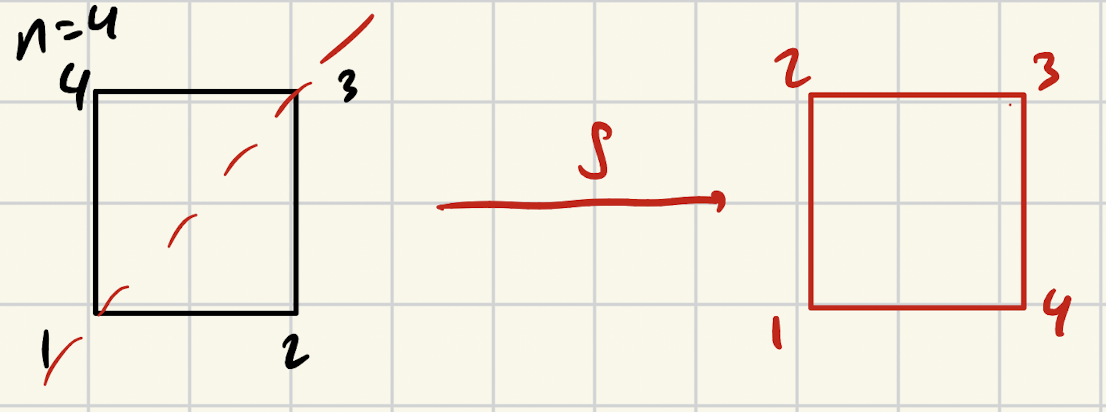
\includegraphics[width= 100pt, center]{/Users/josiahvillarante/GradSchool/Grad-School-Notes/Math210A/CH2/images/Symmetry over vertex 1.png}

    Notice: $1, r, r^2, r^3$ are all distinct. Now consider $s, sr, sr^2, sr^3$ (we read these right-to-left). $sr^3$ is the $270^\circ$ rotation clockwise, then the reflection about the line where vertex $1$ was to the origin.

    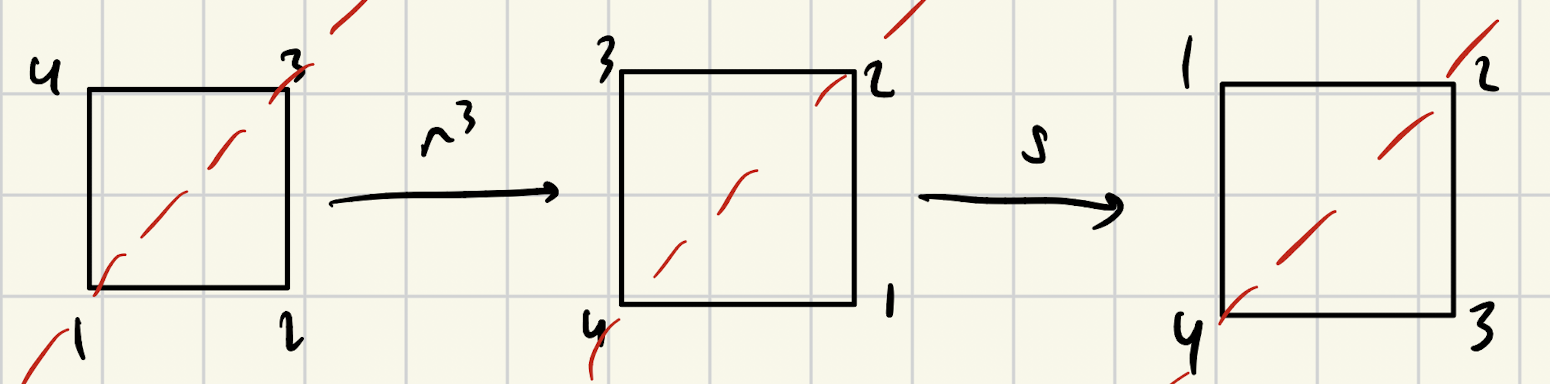
\includegraphics[width= 100pt, center]{/Users/josiahvillarante/GradSchool/Grad-School-Notes/Math210A/CH2/images/sr^3.png}

    Is $s \in \set{1, r, r^2, r^3}?$ No, $s$ fixes vertex $1$ and the only element that fixes vertex $1$ is the identity. But $s \not = 1$, so $s$ is not a rotation. From here, we can deduce that
    $$sr^j \not r^i$$
    for any $0 \leq j \leq 3$ or $0 \leq i \leq 3$ (if it were true that $sr^j = r^i$ for some $i$ and $j$, then $s = r^{i-j}$). Hence $D_{2\dot 4} = \set{1, r, r^2, r^3, s, sr, sr^2, sr^3} = <r, s>/$
\end{example}

In $D_{2n}, n \geq 3,$ we want to show that 
$$D_{2n} = \set{e, r, r^2, r^3, ..., r^{n-1}, s, sr, sr^2, ..., sr^{n-1}}$$
where $s$ is a reflection over the line passing through vertex $1$ and the origin.

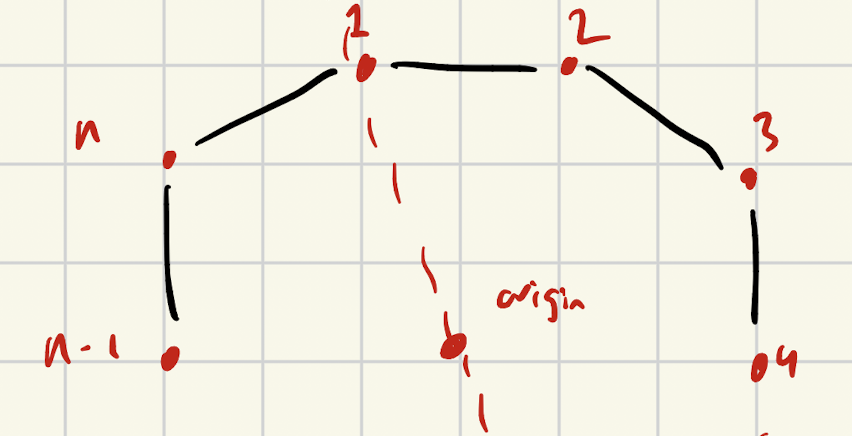
\includegraphics[width= 100pt, center]{/Users/josiahvillarante/GradSchool/Grad-School-Notes/Math210A/CH2/images/n-gon reflection.png}

\begin{enumerate}
    \item Why are all $e, r, r^2, ..., r^{n-1}$ distinct? 
    \begin{align*}
        r^i(1) &= i + 1 \text{ for $0\leq i \leq n -1$ } \\
        r^i(1) &= r^j(1) \\
        \implies i + 1 &= j + 1 \\
        \implies i &= j
    \end{align*}
    so the $r^i$'s are distinct.

    \item $s \not = r^i$ for any $i \in \set{0, ..., n-1}$. $s(1) = 1$ if $r^i(1) = 1,$ we know from part 1 that $i = 0$. That is, $r^i = e$. But $s(2) = n \not = 2 = e(2) \implies s \not = e, s \not = r^i ~\forall 0 \leq i \leq n$

    \item Let's show that $r^i \not = sr^j$ for any $i, j \in \set{0, ..., n-1} = A$.
    Suppose there exists $i,j\in A \st r^i = sr^j$. We define $r^{-1}$ as a counter-clockwise rotation; $r^-1 = r^{n-1}$. This gives 
    \begin{align*}
        r^i &= sr^j \\
        \implies r^{i-j} &= s \\
        \implies r^{i + n-j} &= s
    \end{align*}
    where we adjust $(i + n-j) \mod n$ as needed. This contradicts $s \not \in \set{e, r, r^2, ..., r^{n-1}}$. Hence $r^i \not = sr^j$ for any $i, j \in A$.

    \item Show that $sr^i \not = sr^j$ for any $i \not = j$ in $A$.
    For the sake of contradiction, suppose there exists $i, j \in A \st sr^i = sr^j.$ Then 
    \begin{align*}
        s^2r^i &= s^2r^j \\
        \implies er^i &= er^j \\
        \implies r^i &= r^j
    \end{align*}
    This contradicts $i \not = j$.
    \begin{align*}
        &D_{2n} = \set{e, r, r^2, ..., r^{n-1}, s, sr, sr^2, ..., sr^{n-1}} \\ 
        &sr \not = rs \\
        (s\circ r)(1)=s(r(1)) &&(r \circ s)(1)=r(s(1)) \\
        = s(2)  &&= r(1)  \\
        = n  &&= 2
    \end{align*}
    But $sr = r^{-1}s$. If $sr(1) = r^{-1}s(1)$ and $sr(2) = r^{-1}s(2),$ then $sr = r^{-1}s.$ It can be shown inductively that $sr^i = r^{-i}s ~\forall i \in \Z.$
\end{enumerate}

Let $ x\in G$ and $H \leq G$. If $x \in H$, then $<x> \leq H$. In some sense, $<x>$ is the smallest subgroup of $G$ which contains $x$. "Smallest" refers to containment.

\begin{proposition}
    \label{prop8}
    If $\mathcal{A}$ is any collection of subgrops of a group $G$, then $\bigcap \limits_{H \in \mathcal{A}} H \leq G.$
\end{proposition}

\begin{proof}
    HW
\end{proof}

\begin{definition}[Generating Sets] \leavevmode \\
    If $A$ is any subset of the group $G$, define
    $$<A> = \bigcap \limits_{H \leq G, A \subseteq H} H$$
    This is called the subgroup of $G$ generated by $A$. $A$ is called the generating set. 
\end{definition}

Notice that in the notation of prop \ref{prop8}
$$\mathcal{A} = \set{H \leq G : A \subseteq H} \text{(nonempty as $G \in A$ since $G\leq G$ and $A \subseteq G$)}$$
We will show that $<A> $ is the unique minimal element of $\mathcal{A}$.

We know that $A \subseteq H ~~\forall H \in \mathcal{A}.$ Thus $A \subseteq <A>, $ so $<A> \in \mathcal{A}$.
Let $K \in \mathcal{A}.$ We know that 
$$\bigcap \limits_{H\in \mathcal{A}} H \leq K$$
That is, $<A> \leq K.$ Hence, $<A>$ is minimal with respect to inclusion. When $A$ is finite, that is
$$A = \set{a_1, ..., a_n} \text{ for } n \in \N$$
then we write 
$$<A> = <a_1, a_2, ..., a_n>$$
This is a more concrete verion of the previous set $<A> = \bigcap \limits_{H \leq G, A \subseteq H} H.$
Denote
$$\overline{A} = \set{a_1^{\epsilon_1} a_2^{\epsilon_2} ... a_n^{\epsilon_n} : n \in \N, \epsilon_i = \pm 1, a_i \in A}$$

In $D_{2n}$, $x \in <r,s>$ could look like
$$rssssssr^{-1}s^{-1}srrs^{-1}rr^{-1}s = r^2$$

\begin{proposition}
    $<A> = \overline{A}$.
\end{proposition}
\newpage

\section{Quotient Groups and Homomorphisms}
Let $G$ be a group and $N\leq G$. Define a relation on $G$ by 
$$a \sim b \iff a^{-1}b \in N$$
It is straightforward to verify that this is an equivalence relation on $G$. For $a \in G$, the equivalence class of $a$ is
\begin{align*}
    \set{b \in G : a \sim b} &= \set{b \in G : a^{-1}b \in N} \\
    &= \set{b \in G : a^{-1}b = n \text{ for } n \in N} \\
    &= \set{b \in G : b = an \text{ for } n \in N} \\
    &= \set{an : n \in \N} \\
    aN := \set{an : n \in N}
\end{align*}

\begin{definition} [Coset] \leavevmode \\
    For a subgroup $N$ of $G$ and $g \in G$, let
    \begin{align*}
        gN &= \set{gn : n \in N} \\
        Ng &= \set{ng : n \in N}
    \end{align*}
    be called the left coset and right coset of $N$ in $G$, respectively. Any element of a coset is called a representative of that coset. We will denote the set of all left cosets of $N$ in $G$ by $G/N$ (read $G$ modulo $N$ or $G$ mod $N$).
\end{definition}

\begin{proposition}
    \label{prop4}
    Let $N \leq G$. $G/N$ forms a partition of $G$. For all $a,b \in G$, 
    $$aN = bN \iff \text{$a$ and $b$ are representatives of the same coset.}$$
\end{proposition}

\begin{proof}
    Since we have recognized left cosets as the equivalence classes induced by an equivalence relation, they form a partition. That is,
    $$G = \bigcup_{g \in G}gN$$
    $$\forall g_1, g_2 \in G ~~g_1N = g_2N \iff g_1 N \cap g_2 N \not = \emptyset$$
    Suppose $a^{-1}b \in N$. Then $a^{-1}b = n$ for some $n \in N$. It follows that $b = an \in aN$ so $ b\in aN.$ Since $N$ is a subgroup, $1 \in N$ hence $b\cdot 1 \in bN$. It follows that $aN \cap bN \not = \emptyset \implies aN = bN.$

    Now assume $aN = bN$. Then $an = b$ for some $n \in N$. It follows that $n = ba^{-1} \in N$. Finally, we have
    \begin{align*}
        aN = bN &\iff a^{-1}b \in N \\ 
        &\iff b \in aN \\ 
        &\iff b \in aN \text{ and } a \in aN \\
        &\iff a \text{ and } b \text{ are representatives of } aN \text{(or $bN$)}
    \end{align*}
    \qed
\end{proof}

\begin{proposition}
    \label{prop5}
    Let $N\leq G.$
    \begin{enumerate}
        \item The operation on $G/N$ described by $aN \cdot bN = (ab)N ~~\forall a, b \in G$ is well-defined if and only if $gng^{-1} \in N ~~\forall g \in G, n \in N$
        \item If the operation above is well-defined, then $G/N$ defines a group, where 
        \begin{align*}
            1 \cdot N \text{ is the identity } \\
            (gN)^{-1} = g^{-1}N ~\forall g \in G
        \end{align*}
    \end{enumerate}
\end{proposition}

\begin{proof}
    1. $(\impliedby)$ Suppose $gng^{-1} \in N ~\forall g \in G, n \in N$. Let $a, a_1 \in aN$ and $b, b_1 \in bN$. We want to show that 
    $$abN = a_1b_1N$$
    $a_1 = an$ and $b_1 = bm$ for some $n,m \in N$. Note that $a_1b_1 \in abN \iff a_1b_1N = abN,$ so we will prove the former.
    \begin{align*}
        a_1b_1 = (an)(bm) &= a(bb^{-1})nbm \\
        &= ab(b^{-1}nb)m
    \end{align*}
    by assumption, $b^{-1}n(b^{-1})^{-1} \in N$ so it follows that $a_1b_1 = abn_1m$ where $n_1 \in N$. Since $N$ is a subgroup of $G$, $n_1m \in N$, call it $n_2$. Thus $a_1b_1 = abn_2$ where $n_2 \in N$. That is, $a_1b_1 \in abN$, proving our result ($a_1b_1N = abN$).
    
    2. Suppose the operation is well-defined. We want to show $G/N$ is a group.
    \begin{description}
        \item[Associativity: ] Let $aN< bN< cN \in G/N$ ($a,b,c \in G$). Then 
        \begin{align*}
            aN(bNcN) &= aN\left((bc)N\right) \\
            &= a(bc)N \\
            &=(ab)cN \\
            &=\left((ab)N\right)cN \\
            &= (aNbN)cN
        \end{align*}
        \item[Identity, Closure, and Inverses: ] Let $aN \in G/N$ be given. Since $B$ is a group, $1 \in G$ and thus
        $$1N \in G/N$$
        and
        $$(aN)(1N) = (a1)N = aN$$
        Also,
        \begin{align*}
            \begin{rcases*}
                a \in G \\
                G \text{ is a group}
            \end{rcases*} \implies a^{-1} \in G \implies a^{-1}N \in G/N
        \end{align*}
        and so
        \begin{align*}
            (aN)(a^{-1}N) &= (aa^{-1})N \\
            &= 1N \\
            &= (a^{-1}a)N \\
            &= (a^{-1}N)(aN)
        \end{align*}
    \end{description}
    \qed
\end{proof}

$G/N$ will be a group when $N$ has that nice property, detailed in the following definition.

\begin{definition}[Normal Subgroup] \leavevmode \\
    A subgroup $N$ of $G$ is called normal in $G$ if every element of $g$ normalizes $N$. That is, $N$ is normal in $G$ if 
    $$gNg^{-1} = N ~~\forall g \in G$$
    If $N$ is a normal subgroup of $G$, then we write $N \nsubgroup G$.
\end{definition}

\begin{theorem}[Characterizations of Normal Subgroups] \leavevmode \\
    \label{thm6}
    The $N \leq G$. The following are equivalent:
    \begin{enumerate}
        \item $N \nsubgroup G$
        \item $N_G(N) = G$
        \item $gN = NG ~~\forall g \in G$
        \item The operation "coset multiplication" is well-defined 
        \item $gNg^{-1} \subseteq N ~~\forall g \in G$
    \end{enumerate}
\end{theorem}

\begin{example}
    Checking that a subgroup is normal is not practical using the definition. We would need to check that $gng^{-1} \in N ~~\forall g \in G, n \in N$. If a subgroup is finitely generated, it suffices to check that the generators map back to the subgroup by conjugating.

    Let $G = D_{16}$. Is $<s>$ normal in $D_{16}$? We need to examine $gsg^{-1}$ for an arbitrary $g \in D_{16}$. Letting $g = s^ir^j$ where $i \in \set{0,1}$ and $j \in \set{0, ..., 7}$. Then 
    \begin{align*}
        gsg^{-1} &= (s^ir^j)s(s^ir^j)^{-1} \\
        &= s^ir^jsr^{-j}s^{-i} \\
        &= r^jsr^{-j} \text{  (when $i=0$)}\\
        &= r^jr^{-j}s \text{  ($sr^{-j} = r^{-(-j)}s = r^js$)} \\
        &= r^{2j}s
    \end{align*}
    When $j=1$, this gives that $gsg^{-1} = r^2s \not \in <s>$ since this would imply that $r^2$ is either the identity or $s$ ($r^2s = 1\implies r^2 = s, ~r^2s =s \implies r^2 = 1$) which is a contradiciton.
\end{example}

\begin{theorem}[Big Theorem] \leavevmode \\
    \label{thmBIG}
    A subgroup $N\leq G$ is normal in $G$ if and only if it is the kernel of some homomorphism.
\end{theorem}

\begin{proof}
    ($\impliedby$) HW 

    ($\implies$)Suppose $N \nsubgroup G$. Let's define 
    \begin{align*}
        \pi : G &\to G/N \\
        \pi(g) &= gN ~~\forall g \in G
    \end{align*}
    Let $g_1, g_2 \in G$. Then 
    \begin{align*}
        \pi(g_1g_2) &= (g_1g_2)N \\
        &= (g_1N)(g_2N) \\
        &= \pi(g_1)\pi(g_2)
    \end{align*}
    Hence, $\pi$ is a homomorphism. It remains to show that $\ker\pi = N.$ Note that 
    \begin{align*}
        \ker\pi &= \set{g \in G : \pi(g) = 1N} \\
        &= \set{g \in G : gN = 1N} \\
        &= \set{g \in G : g \in 1N} \\
        &= \set{g \in G : g \in N} \\
        &= N
    \end{align*}
    completing the proof.
    \qed
\end{proof}

\begin{definition}[Natural Projection Homomorphism] \leavevmode \\
    Let $N\nsubgroup G$. The homomorphism
    \begin{align*}
        \pi: G &\to G/N \\
        \pi(g) &= gN
    \end{align*}
    is called the natural projection (homomorphism) of $G$ onto $G/N$.
\end{definition}

If $\overline{H} \leq G/N$, the complete preimage of $\overline{H}$ is $\pi^{-1}(\overline{H}).$

\begin{note}
    If $\overline{H} \leq G/N$, then 
    $$N \leq \pi^{-1}(\overline{H})$$
    Since $1N \in \overline{H}$, we have $N = \ker \pi = \pi^{-1}(1N) \subseteq \pi^{-1}(\overline{H})$.
\end{note}

$Q_8$: we have that $<-1>$ is a normal subgroup, so $Q_8/<-1>$ is a group consisting of $1<-1>, i<-1>, j<-1>, k<-1>$ 
$$(i<-1>)^2 = i^2<-1> = -1<-1> = 1<-1>$$
so, $Q_8/<-1> \cong V_4$.
\begin{align*}
    \left<i<-1>\right> &\cong Q_8/<-1> \\
    \left<i<-1>\right> &= \set{i<-1>, 1<-1>} = \overline{H} \\
    \pi^{-1}(\overline{H})&= \set{g \in Q_8 : \pi(g) \in \overline{H}}
\end{align*}
\begin{align*}
    \pi(1) &= 1<-1> \in \overline{h} &&\pi^{-1}(\overline{H}) = \set{1, i, -1, -i} \\
    \pi(i) &= i<-1> \in \overline{H} \\
    \pi(-1) &= -1<-1> = 1<-1> \in \overline{H} \\
    \pi(-i) &= -i<-1> = i<-1> \in \overline{H}
\end{align*}
\newpage

\end{document}